\documentclass[aspectratio=169,10pt]{beamer}
\usetheme{metropolis}
\usepackage{booktabs}
\usepackage{amsmath,amssymb}
\usepackage{graphicx}
\usepackage{tikz}
\usepackage{xcolor}

\definecolor{accent}{HTML}{e74c3c}
\definecolor{good}{HTML}{27ae60}
\definecolor{bad}{HTML}{e74c3c}
\setbeamercolor{alerted text}{fg=accent}

\title{Token-Importance Guided PPO for Math Reasoning}
\subtitle{Adaptive Intensity Weighting: When, Why, and Where It Helps}
\author{Gurusha Juneja}
\date{March 2026}

\begin{document}

\maketitle

% ============================================================
% SLIDE 1: The Problem
% ============================================================
\begin{frame}{The Problem: Not All Tokens Are Equal in RLHF}

Standard PPO treats every token equally in the policy gradient:
\[
\mathcal{L}_{\text{PPO}} = \frac{1}{T}\sum_{t=1}^{T} \min\!\bigl(r_t \hat{A}_t,\; \text{clip}(r_t)\,\hat{A}_t\bigr)
\]

\textbf{But tokens contribute unequally:}
\begin{itemize}
    \item \textit{``The movie was \alert{surprisingly} good''} --- the adjective carries the reward signal
    \item \textit{``\alert{72} is the answer''} --- the final number is what matters in math
    \item Function words (``the'', ``is'', ``a'') are noise in the gradient
\end{itemize}

\vspace{0.3cm}
\textbf{Question:} Can we weight tokens by importance to get \textit{faster learning} and \textit{lower KL divergence}?

\vspace{0.3cm}
\textbf{TI-DPO} (Yang et al., 2025) showed this works for DPO. \textbf{Does it transfer to PPO?}
\end{frame}

% ============================================================
% SLIDE 2: Why This Is Hard
% ============================================================
\begin{frame}{Why This Is Harder Than It Looks}

\textbf{DPO vs PPO --- a fundamental difference:}

\begin{columns}
\begin{column}{0.48\textwidth}
\textbf{DPO (offline)}
\begin{itemize}
    \item Paired (chosen, rejected) sequences
    \item Single pass over data
    \item Bias doesn't accumulate
    \item Token importance = ``which tokens differ between chosen/rejected?''
\end{itemize}
\end{column}
\begin{column}{0.48\textwidth}
\textbf{PPO (online)}
\begin{itemize}
    \item Single sequence + scalar reward
    \item Hundreds of gradient steps
    \item \alert{Bias accumulates over training}
    \item Token importance = ??? (no contrastive signal)
\end{itemize}
\end{column}
\end{columns}

\vspace{0.5cm}
Importance weighting introduces a \alert{persistent bias} in the PPO gradient that compounds over training steps.

\end{frame}

% ============================================================
% SLIDE 3: TI-DPO Background
% ============================================================
\begin{frame}{Background: TI-DPO (Yang et al., 2025)}

Token-Importance guided DPO weights the preference loss per-token:
\[
\mathcal{L}_{\text{TI-DPO}} = -\log\sigma\!\Bigl(\beta\sum_t \alert{w(t)}\bigl[\log\pi(a_t^w|s_t) - \log\pi(a_t^\ell|s_t)\bigr]\Bigr)
\]

\textbf{Their importance scoring methods:}

\begin{table}
\small
\begin{tabular}{lll}
\toprule
Method & Signal & Cost \\
\midrule
Gradient & $\|\nabla_{\text{emb}}\|_1$ per token & 1 backward \\
Attention & Mean attention received & 1 forward \\
Hybrid & Gradient + Gaussian prior & 1 backward + 1 forward \\
TD Error & $|V(s_t) - V(s_{t+1}) - r_t|$ & Free \\
\bottomrule
\end{tabular}
\end{table}

Works well for DPO: +2-5\% on preference benchmarks.

\textbf{Our goal:} Adapt this to PPO for math reasoning (GSM8K).

\end{frame}

% ============================================================
% SLIDE 4: Phase 1 --- Porting to PPO
% ============================================================
\begin{frame}{Phase 1: Direct Port of TI-DPO Methods to PPO}

We weight the PPO clipped surrogate per-token:
\[
\mathcal{L} = \frac{1}{T}\sum_t \alert{w(t)} \cdot \min\!\bigl(r_t \hat{A}_t,\;\text{clip}(r_t)\hat{A}_t\bigr)
\]

\textbf{Result: Paper methods \alert{underperform} vanilla PPO.}

\begin{table}
\small
\begin{tabular}{lccc}
\toprule
Method & Reward (Q4) & KL (Q4) & KL-Efficiency \\
\midrule
PPO baseline (uniform) & \textbf{0.850} & 0.043 & 19.9 \\
Paper: Hybrid+Triplet & 0.779 & 0.024 & 32.7 \\
\bottomrule
\end{tabular}
\end{table}

The DPO-derived signals (gradient attribution, attention) don't provide useful importance information in PPO --- there's no contrastive pair to derive importance from.

\end{frame}

% ============================================================
% SLIDE 5: Phase 2 --- PPO-Native Methods
% ============================================================
\begin{frame}{Phase 2: PPO-Native Importance Methods}

Derive importance from quantities \textit{naturally available} in PPO:

\begin{columns}
\begin{column}{0.55\textwidth}
\textbf{Advantage magnitude:}
\[w(t) = \frac{|\hat{A}(t)|}{\text{mean}(|\hat{A}|)}\]
Large advantage $\to$ strong reward signal $\to$ focus here.

\vspace{0.3cm}
\textbf{Entropy:}
\[w(t) = \frac{H(\pi(\cdot|s_t))}{\text{mean}(H)}\]
High entropy $\to$ model is uncertain $\to$ room to learn.

\vspace{0.3cm}
Both are \textbf{free} --- computed from existing logits/advantages.
\end{column}
\begin{column}{0.42\textwidth}
\textbf{Early results (100 episodes):}
\begin{table}
\small
\begin{tabular}{lc}
\toprule
Method & R(Q4) \\
\midrule
Entropy & 0.872 \\
$|$Advantage$|$ & 0.870 \\
PPO baseline & 0.791 \\
\bottomrule
\end{tabular}
\end{table}

\vspace{0.2cm}
\textcolor{good}{\textbf{+10\% over baseline!}}

\vspace{0.2cm}
But wait\ldots
\end{column}
\end{columns}

\end{frame}

% ============================================================
% SLIDE 6: The Degradation
% ============================================================
\begin{frame}{The Catch: Every Fixed-Intensity Method Degrades}

\textbf{At 150 episodes, the picture reverses:}

\begin{table}
\small
\begin{tabular}{lccc}
\toprule
Method & R(Q4) at ep 100 & R(Q4) at ep 150 & Trend \\
\midrule
PPO baseline & 0.791 & \textbf{0.850} & $\uparrow$ keeps improving \\
Entropy & \textbf{0.872} & 0.797 & \textcolor{bad}{$\downarrow$ degraded} \\
$|$Advantage$|$ & 0.870 & 0.785 & \textcolor{bad}{$\downarrow$ degraded} \\
\bottomrule
\end{tabular}
\end{table}

\vspace{0.3cm}

\textbf{Pattern:} Importance weighting helps early ($<$100 steps), then hurts.

This is not a bug in any specific method --- it's a \alert{fundamental property} of non-uniform weighting in online policy gradient.

\end{frame}

% ============================================================
% SLIDE 7: The Math --- Bias-Variance Tradeoff
% ============================================================
\begin{frame}{The Key Insight: Bias-Variance Tradeoff}

The PPO gradient with importance weights:
\[
g_w = \mathbb{E}_t\bigl[w(t) \cdot \nabla\log\pi(a_t|s_t) \cdot \hat{A}_t\bigr]
\]

\textbf{Bias of this estimator:}
\[
\text{Bias} = \mathbb{E}[g_w] - \mathbb{E}[g] = \text{Cov}(w, f) \neq 0
\]
where $f = \nabla\log\pi \cdot \hat{A}$.

\vspace{0.3cm}

\begin{columns}
\begin{column}{0.48\textwidth}
\textbf{Early training:}
\[
\underbrace{\text{Var}(g)}_{\text{large}} \gg \underbrace{|\text{Bias}|}_{\text{small}}
\]
Importance reduces variance $\to$ \textcolor{good}{helps}
\end{column}
\begin{column}{0.48\textwidth}
\textbf{Late training:}
\[
\underbrace{|\text{Bias}|}_{\text{accumulated}} \gg \underbrace{\text{Var}(g)}_{\text{small}}
\]
Bias dominates $\to$ \textcolor{bad}{hurts}
\end{column}
\end{columns}

\vspace{0.3cm}
\textbf{This explains why TI-DPO works} (single pass, no accumulation) \textbf{but TI-PPO doesn't} (online, hundreds of steps).

\end{frame}

% ============================================================
% SLIDE 8: Our Solution --- AITI
% ============================================================
\begin{frame}{Our Solution: Adaptive Intensity Token Importance (AITI)}

\textbf{Decay the importance intensity over training:}
\[
w_{\text{AITI}}(t) = 1 + \alert{\varepsilon(\text{step})} \cdot \bigl(s(t) - 1\bigr)
\]

\begin{itemize}
    \item $s(t)$ = any base importance score (advantage, entropy, etc.)
    \item $\varepsilon$ decays from 1 $\to$ 0 over training
    \item $\varepsilon = 1$: full importance weighting (max variance reduction)
    \item $\varepsilon = 0$: uniform PPO (zero bias)
\end{itemize}

\vspace{0.3cm}
\textbf{Analogy:} Learning rate scheduling controls \textit{step size}. AITI controls \textit{gradient quality}.

\begin{table}
\small
\begin{tabular}{lcc}
\toprule
Phase & Learning Rate & AITI Intensity ($\varepsilon$) \\
\midrule
Early & High (explore) & High (reduce variance, accept bias) \\
Late & Low (fine-tune) & Low (reduce bias, accept variance) \\
\bottomrule
\end{tabular}
\end{table}

\end{frame}

% ============================================================
% SLIDE 9: MOAI
% ============================================================
\begin{frame}{MOAI: MSE-Optimal Adaptive Intensity}

Instead of a fixed decay schedule, \textbf{compute optimal $\varepsilon^*$ per step}:

\[
\varepsilon^* = \arg\min_\varepsilon\; \text{MSE}(g_\varepsilon) = \arg\min_\varepsilon\; \bigl[\text{Bias}(\varepsilon)^2 + \text{Var}(\varepsilon)\bigr]
\]

\textbf{Closed-form solution} (with monotone constraint $\varepsilon^* \leq \varepsilon^*_{\text{prev}}$):

\[
\varepsilon^* = \text{clip}\!\left(\frac{-C}{2\rho}, 0, \varepsilon_{\text{prev}}\right)
\]

where $C = \text{Cov}(s, f)$ and $\rho = \text{Var}(s) \cdot \mathbb{E}[f^2]$, estimated via EMA.

\vspace{0.3cm}
\textbf{Key discovery:} MOAI converges to $\varepsilon^* \approx 0.3$--$0.5$, \textit{not} zero.

$\Rightarrow$ The optimal policy is \textbf{permanent partial weighting}, not full decay to uniform.

\end{frame}

% ============================================================
% SLIDE 10: Synthetic Benchmark Results
% ============================================================
\begin{frame}{Results: Synthetic Reward Benchmark}

\begin{table}
\small
\begin{tabular}{lcccc}
\toprule
Method & Reward (Q4) & KL (Q4) & KL-Efficiency & Pareto? \\
\midrule
\textbf{MOAI-Adv mono} & \textbf{0.880} & 0.056 & 15.7 & \textcolor{good}{\textbf{YES}} \\
\textbf{AITI-Advantage} & 0.874 & \textbf{0.031} & \textbf{28.4} & \textcolor{good}{\textbf{YES}} \\
PPO baseline & 0.859 & 0.028 & 30.4 & YES \\
TI-DPO Hybrid+Triplet & 0.779 & 0.024 & 32.7 & dominated \\
Advantage (fixed) & 0.785 & 0.107 & 7.3 & dominated \\
Entropy (fixed) & 0.797 & -0.504 & 1.6 & dominated \\
\bottomrule
\end{tabular}
\end{table}

\vspace{0.3cm}
\begin{itemize}
    \item MOAI: \textbf{highest reward} (+2.4\% over baseline)
    \item AITI: \textbf{best reward/KL tradeoff} (2.5$\times$ lower KL than baseline)
    \item Both \textbf{Pareto-dominate} uniform PPO
    \item Fixed-intensity methods all dominated (confirming the bias theory)
\end{itemize}

\end{frame}

% ============================================================
% SLIDE 11: GSM8K Setup
% ============================================================
\begin{frame}{GSM8K: Real Math Reasoning Benchmark}

\textbf{Setup:}
\begin{itemize}
    \item Model: Qwen2.5-1.5B-Instruct + LoRA (r=16)
    \item Task: GSM8K grade-school math (7,473 train / 1,319 test)
    \item Reward: Binary (+1 correct, -1 wrong) via $\backslash$boxed\{\} extraction
    \item Training: 200 episodes, batch size 4, 4 PPO epochs
    \item Eval: Greedy decoding on full test set
\end{itemize}

\vspace{0.3cm}
\textbf{Implementation challenges we solved:}
\begin{enumerate}
    \item \alert{Value head fp16 overflow} --- NaN after 1 step $\to$ float32 value head
    \item \alert{Logprob fp16 underflow} --- KL$=$0 always $\to$ float32 log-softmax
    \item \alert{Answer extraction} --- model truncated mid-answer $\to$ $\backslash$boxed\{\} prompt
    \item \alert{Chat template} --- 55\% $\to$ 65\% base accuracy by using proper format
    \item \alert{Overfitting} --- pool of 500 $\to$ full 7,473 training set
\end{enumerate}

\end{frame}

% ============================================================
% SLIDE 12: GSM8K Training Results
% ============================================================
\begin{frame}{GSM8K: Training Curves}

\begin{columns}
\begin{column}{0.55\textwidth}
\textbf{8 methods, 200 episodes, 8 GPUs:}
\begin{itemize}
    \item PPO baseline, AITI (adv, entropy), MOAI (adv, entropy) $\times$ 2 EMA settings, fixed advantage
    \item All start at $\sim$75\% (base model accuracy)
    \item Training accuracy: 64--68\% across methods
    \item MOAI-Entropy has \textbf{lowest KL} (0.001) with competitive accuracy
\end{itemize}

\vspace{0.3cm}
\textbf{Batch size finding:}

At bs=1, AITI-Advantage gives \textbf{+4.6\%} over baseline (59.3\% vs 54.7\%).

At bs=8, the gap vanishes.

$\Rightarrow$ Token importance = \textbf{variance reducer}, most valuable in high-variance (small batch) regimes.
\end{column}
\begin{column}{0.43\textwidth}
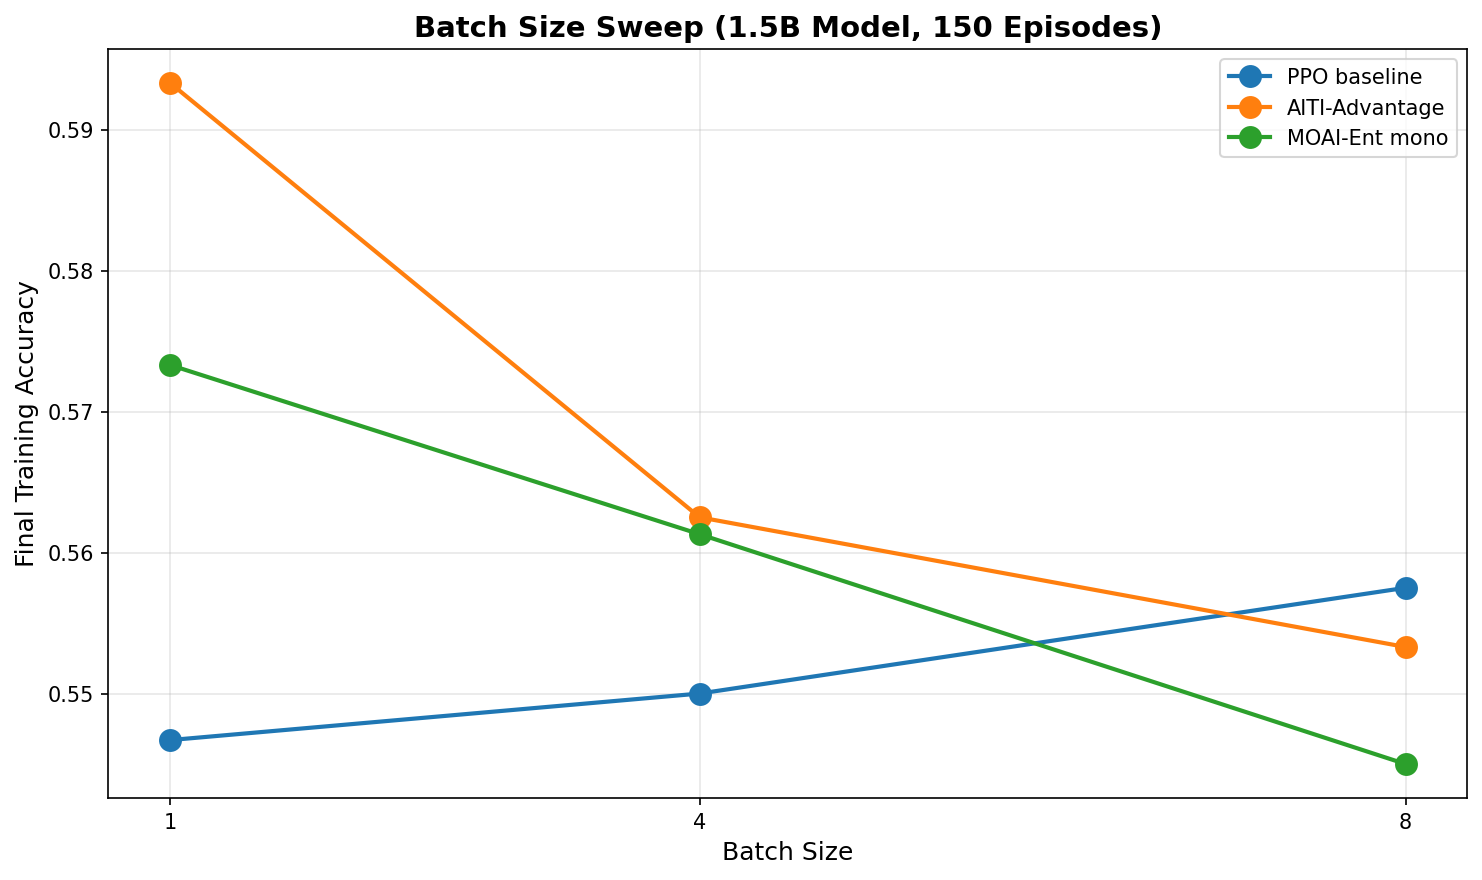
\includegraphics[width=\textwidth]{plots/gsm8k_batchsize_sweep.png}
\end{column}
\end{columns}

\end{frame}

% ============================================================
% SLIDE 13: Epsilon Sweep
% ============================================================
\begin{frame}{Epsilon Sweep: Fixed vs Adaptive Intensity}

\begin{center}
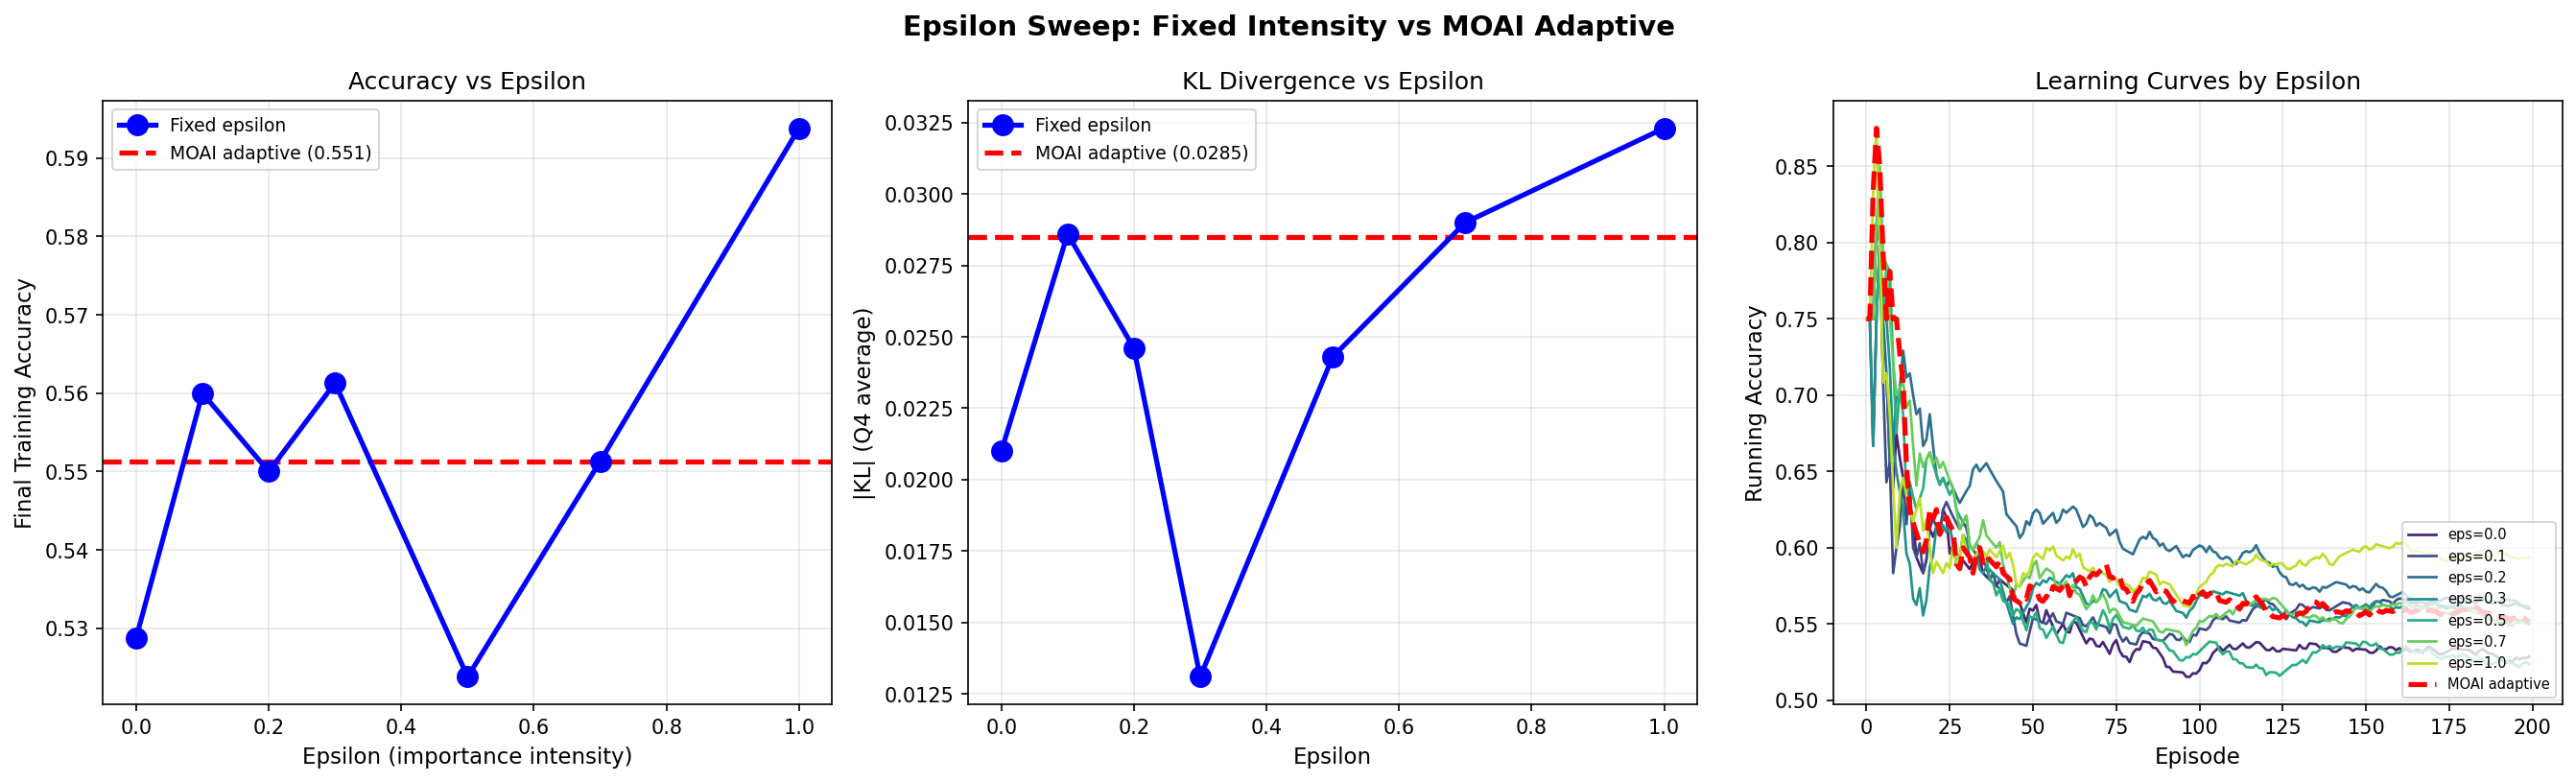
\includegraphics[width=0.85\textwidth]{plots/gsm8k_epsilon_sweep.png}
\end{center}

\begin{itemize}
    \item Accuracy vs $\varepsilon$ is \textbf{non-monotonic} --- both $\varepsilon=0$ and $\varepsilon=0.5$ are local minima
    \item MOAI adaptive (red line) lands at a reasonable middle ground
    \item The optimal fixed $\varepsilon$ varies by task --- adaptive selection avoids this tuning
\end{itemize}

\end{frame}

% ============================================================
% SLIDE 14: Takeaways
% ============================================================
\begin{frame}{Key Takeaways}

\begin{enumerate}
    \item \textbf{Token importance weighting in PPO has a bias-variance tradeoff}
    \begin{itemize}
        \item Fixed intensity: helps early, hurts late (bias accumulates)
        \item This explains why TI-DPO (offline) works but direct TI-PPO (online) doesn't
    \end{itemize}

    \vspace{0.2cm}
    \item \textbf{AITI solves this by decaying importance intensity}
    \begin{itemize}
        \item Variance reduction early + unbiased gradients late
        \item Pareto-dominates PPO baseline on synthetic rewards
    \end{itemize}

    \vspace{0.2cm}
    \item \textbf{MOAI computes optimal $\varepsilon^*$ in closed form}
    \begin{itemize}
        \item Discovers that permanent partial weighting ($\varepsilon \approx 0.3$--$0.5$) beats full decay
    \end{itemize}

    \vspace{0.2cm}
    \item \textbf{On real tasks (GSM8K), the benefit is regime-dependent}
    \begin{itemize}
        \item Strongest at \textbf{small batch sizes} (high gradient variance)
        \item Diminishes at larger batch sizes where variance is already low
        \item Proper evaluation pipeline critical: chat template, answer extraction, full training set
    \end{itemize}
\end{enumerate}

\end{frame}

% ============================================================
% SLIDE 15: Future Directions
% ============================================================
\begin{frame}{Future Directions}

\begin{columns}
\begin{column}{0.48\textwidth}
\textbf{Scaling up:}
\begin{itemize}
    \item Larger models (3B, 7B) where PPO gap over base is bigger
    \item More training episodes (1000+) to see full bias-variance dynamics
    \item Harder benchmarks (MATH, competition-level problems)
\end{itemize}

\vspace{0.3cm}
\textbf{Methodological:}
\begin{itemize}
    \item Per-layer importance (not just per-token)
    \item Importance-weighted KL penalty (not just the policy loss)
    \item Combine with other RL tricks (GRPO, reward shaping)
\end{itemize}
\end{column}
\begin{column}{0.48\textwidth}
\textbf{Theoretical:}
\begin{itemize}
    \item Tighter bounds on the bias-variance crossover point
    \item Connection to importance sampling in off-policy RL
    \item Optimal decay schedule derivation (beyond MSE criterion)
\end{itemize}

\vspace{0.3cm}
\textbf{Practical insight:}

Token importance is a \textbf{variance reduction technique}. Like all variance reduction, it matters most when variance is the bottleneck --- small batches, noisy rewards, early training.
\end{column}
\end{columns}

\end{frame}

\end{document}
